\chapter{Results}
In the following chapter the result of physics through spherical decomposition will
be discussed and performance testing will be presented.

\section{Performance}
Since different shaders is impacted differently by different problems a few performance
test-series has been performed and will be discussed below.
For all tests, cubes have been used as the object being approximated and they
are being dropped into a bin consiting of static particles. For complete data collected and
settings used see appendix~\ref{app:test}.

The times presented for velocity and impulse (who are both iterated ten times per update)
 are the total time for all ten iterations.

\subsection{Number of particles per body}
Increasingly fine decomposition lead to more particles per body.
For this test the number of particles per body increase for each series and is
compensated by adding fewer bodies so that the number of particles in the system
in total is kept constant. For all three series some particles from the bin had to be
either added or removed to keep the total equal between the tests.
\begin{figure}[H]
  \centering
  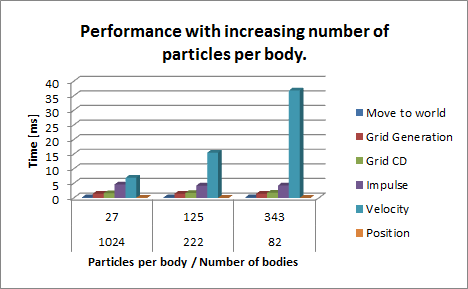
\includegraphics[width = 0.8\textwidth]{particlePerBody.png}
  \caption{Chart of performance of each of the shader steps for increasing number of particles per body.}
  \label{fig:particlePerBody}
\end{figure}
As we can see the velocity shader scales very poorly with the number of particles
within a body. This is not surprising as the shader performs a gather scheme for
summation of the impulses. The shader will perform a number of global reads proportional
against the number of particles in the body per thread.

\subsection{Increasing number of static particles}
For this test we let the number of static particles in the simulation increase
by increasing the dimensions of the bin (box).

\begin{figure}[H]
  \centering
  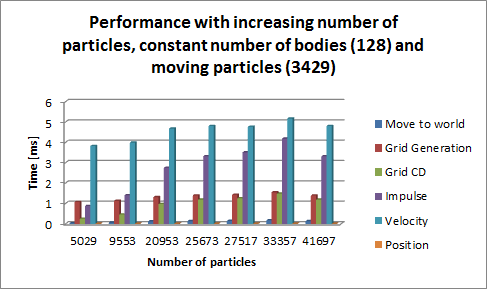
\includegraphics[width = 0.8\textwidth]{staticParticlesIncrease.png}
  \caption{Chart of performance of each of the shader steps for increasing number of static particles.}
\end{figure}

We see some time increase in the grid collision detection and the impulse calculations
and a small increase in the grid generation.
The increase in impulse is not surprising as each particle, even static ones, perform
global reads and writes per particle in the impulse shader step. One could potentially
use a early exit strategy and not perform the impulse calculations for static particles,
however, unless the whole workgroup is static particles one is not guaranteed that
it will net any performance gain as returning threads within a workgroup do not ensure
that new work can be performed.

\subsection{Increasing number of bodies and dynamic particles}
For this test we increase the number of bodies (and particles) in the system.
\begin{figure}[H]
  \centering
  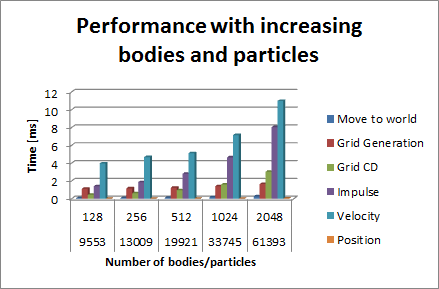
\includegraphics[width = 0.8\textwidth]{bodiesIncrease.png}
  \caption{Chart of performance of each of the shader steps for increasing number of bodies and particles.}
\end{figure}

Here we can see (while difficult to see for move to world and position) an increase in every shader step.
Worst scaling can be seen among the impulse and velocity step. Those shader steps are the two involved
in the stabilization loop and both are executed ten times each per update and optimizations
to these two steps should be prioritized in the future.

\subsection{Increasing grid size}
This test measures the performance of the grid size. For a M-by-M-by-M grid we can detect collisions
effectively on coordinates between -M/2 and +M/2 in each dimension.
\subsection{Increasing number of bodies and dynamic particles}
For this test we increase the number of bodies (and particles) in the system.
\begin{figure}[H]
  \centering
  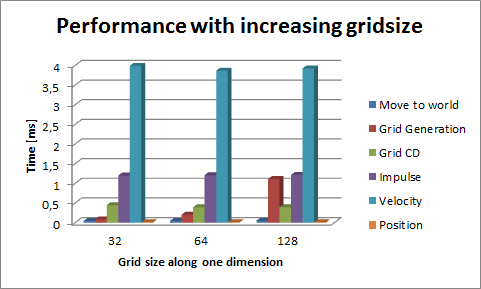
\includegraphics[width = 0.8\textwidth]{gridIncrease.png}
  \caption{Chart of performance of each of the shader steps for increasing number of cells in grid}
\end{figure}

We see that the grid generation scales poorly with the grid size, most likely cubicly
as the number of grid cells increase cubicly and the generation includes the prefix sum and sorting.
We can also note that the grid collision detection does not increase, this is expected since
we still read an equal amount of particles no matter the grid size and the particles are
sorted from the grid generation shader.

\subsection{Increasing cell size}
For this test we increase the domain of the simulation by increasing the cell size instead.
This leads to more particles having to be checked as more and more will end up in
the larger and larger surrounding cells.
\begin{figure}[H]
  \centering
  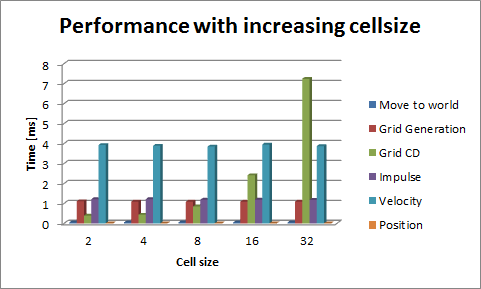
\includegraphics[width = 0.8\textwidth]{cellIncrease.png}
  \caption{Chart of performance of each of the shader steps for increasing cell size}
\end{figure}

It is only the grid collision detection shader which takes a penalty to performances
while changing the cell size, as expected. Note however that for each new series
in this test we get two times the size of the simulation domain in each dimension.
Also note that the time increase from cell size 2 to cell size 8 is only 0.34 ms in total for all shader steps.
This is cheaper than increasing the grid size from 32 to 128, which gives an increase of 0.93 ms.

\subsection{Large scale system}
With a system consisting of 1024 dynamic bodies with 218 particles per body
 and a total of 254348 particles (including
static ones), we get about 103 ms per frame. Which can be compared to Bullet's HACD.
The velocity step is by far the most time consuming step, using around half of the total time with
the impulse step at a second place with about a third of the time. Once again due
to them having to be reiterated 10 times.

\section{Limitations}
\subsection{Per body particle limit}
Currently in the velocity update shader there is a for-loop across all the spheres
belonging to the current body, this is done to gather all the forces from the spheres.
To ensure performance on the GPU one uses unrolling, i.e. the for-loops content is
duplicated for as many iterations as necessary. However on the GPU this mean two
things, we have trouble with dynamic length on the for-loops and there is a upper
bound on how many iterations that are allowed. For the hardware used for the thesis,
this limit is 4096. Therefor the method is currently limited to a maximum of 4096
spheres per body.

\subsection{Tunneling}
Tunneling can occur in the system as no protection against the phenomenon is implemented.
For linear movement such a protection is easily implemented, however with rotations
the protection is slightly more difficult to implement properly. For long thin
objects a smaller time step is recommended.
\subsection{Limited domain}
In addition the domain of the simulation has to be determined before the simulation start
as a uniform spatial partitioning grid is used for the collision detection.

\subsection{False alignment}
Since the method uses spheres as a principal shape the result has a tendency to align
with the grid. A single box consisting of 27 sphere fall on a plane, also made up of spheres
at a slight rotation. All impulses present will drift towards the cube aligning with the
plane at intervals of 90 degrees. The effect would be less apparent with less regularly shaped objects and
is remedied somewhat by friction, albeit not completely.

\section{Comparison to bullet}
\subsection{Concavity}
The method can handle concave results but the current implementations poor scaling
with increased number of particles per body result in a loss against bullets HACD.
It is difficult to not talk about performance in this section as we can get good
concavity results but at the cost of increased voxelization, which in turn affects the
performance.
The performance of HACD with Bullet 2.83 will outperform the spherical decomposition
at equivalent detail.
\subsection{Performance}
In figure~\ref{fig:frameTimeBoxes05}~and~\ref{fig:frameTimeBoxes025}
on pages~\pageref{fig:frameTimeBoxes05}~and~\pageref{fig:frameTimeBoxes025}
we can read out that Bullet can simulate 1000 boxes at around 10 ms per frame.
Spherical decomposition can simulate a box decomposed with 27 spheres at around 15 ms.
The performance is comparable at this level of detail.

Since the velocity and impulse shader steps are iterated
several times for stabilization these steps are quite vital to the performance
of the method. More work could be spent on improving the performance of these shaders,
but one should also investigate if the stabilization iterations could be exchanged for
shock propagation. A sign that this might be the case is the results achieved by~\cite{flex} with nVidia Flex.

For a comparison with HACD, with bullet coming in at 100 ms it now becomes
a question of how many spheres are needed to represent our chosen object.
As presented we can simulate 1024 bodies of 218 particles at 100 ms, which is comparable to
 the implementation Bullet's HACD for 1000 bodies in terms of time. The question is
 if the results are good enough at 218 spheres which is dependent on object detail
 and required detail preservation.

\subsection{Correctness}
Correctness for spherical decomposition depend highly on how finely the model is
decomposed, much like how Bullet's HACD depend on how many vertices is allowed
per model. Boxes with as low as 27 particles looks convincing, but e.g. a Utah Teapot
may need many more particles to produce convincing results.
